\chapter[PRINCIPIOS DE INDUCCIÓN Y DE BUEN ORDEN]{PRINCIPIOS DE \\ INDUCCIÓN Y DE BUEN \\ ORDEN}\label{sec:induction}
\printchaptertableofcontents

Uno de los métodos más usados para realizar demostraciones es el Método de Inducción Matemática. Este fue creado por Blaise Pascal en el siglo XVII, aunque el primer matemático que ofreció una demostración formal mediante el uso explicito de la inducción matemática fue el italiano Franciscus Maurolicus (1494-1575). Maurolicus utilizo la inducción para demostrar que para todo entero positivo $n$
$$1 + 3 + 5 + \cdots + (2n-1) = n^2.$$
Dicho método ha servido para demostrar teoremas en distintas áreas de la matemática; como: geometría, teoría de grafos, teoría de números, análisis combinatorio.

Una manera informal (pero eficaz) de ver y explicar el Principio de Inducción Matemática es mediante fichas de dominó (véase la figura \ref{fig:INDUCCION}). Imaginemos que tenemos fichas de dominó puestas en una hilera infinita. Si empujamos la primer ficha, esta empujará la segunda ficha; la segunda ficha empujará la tercer ficha; la tercer ficha empujara la cuarta ficha; y así sucesivamente hasta que caigan todas las fichas. En este caso, cada ficha representa un número natural.

\newpage
\marginElement{\justify
\includegraphics[width=\linewidth]{Images/ApendiceA/PASCAL.jpeg}
\textbf{Blaise Pascal:} Nacido el 19 de junio de 1623 en Clermont-Ferrand, Francia; fue un genio precoz y de clara inteligencia, pues su entusiasmo juvenil por la ciencia se materializó en importantes y precursoras aportaciones a la física y a las matemáticas. Siendo aún niño, con solo doce años, sin ayuda alguna demostró que la suma de los ángulos de un triángulo es siempre igual a 180°. Pese a su frágil salud y corta vida, murió a los treinta y nueve años, pero su huella quedó grabada en la historia de la física y de la informática.
}
\sideFigure[\label{fig:INDUCCION}Representación del Principio de Inducción]{
\includegraphics[width=\linewidth]{Images/ApendiceA/uuu.pdf}
}

Como preliminar, debemos saber que cualquier proposición se puede clasificar como general o particular. Algunos ejemplos de proposiciones generales son:
\begin{enumerate}
    \item Todos los ciudadanos de México tienen derecho a la educación.
    \item Todos los números que terminan en cero son divisibles entre 5.
\end{enumerate}
Algunos ejemplos de proposiciones particulares son:
\begin{enumerate}
    \item Guinevere tiene derecho a la educación 
    \item 300 es divisible entre 5.
\end{enumerate}
El proceso de obtener una proposición particular de una general se llama \textbf{deducción}. Por ejemplo, si tenemos
\begin{enumerate}
    \item Todos los ciudadanos de México tienen derecho a la educación.
    \item Guinevere es mexicana.
    \item Guinevere tiene derecho a la educación.
\end{enumerate}
entonces de la proposición general (1), junto con la proposición particular (2), se obtiene la proposición particular (3).

El proceso de obtener proposiciones generales de proposiciones particulares se llama \textbf{inducción}. El razonamiento inductivo puede conducir a conclusiones falsas así como a verdaderas. Por ejemplo, si tenemos
\begin{enumerate}
    \item 300 es divisible entre 5.
    \item Todos los números que terminan en cero son divisibles entre 5.
\end{enumerate}
entonces la proposición general (2), obtenida de la proposición particular (1), es verdadera. Pero, si consideramos
\begin{enumerate}
    \item 300 es divisible entre 5.
    \item Todos los números con tres cifras son divisibles entre 5.
\end{enumerate}
entonces la proposición general (2), deducida de la proposición particular (1), es falsa.

\begin{Problem}
    Calcular la suma de los primeros $n$ números impares. \\
    \solucion Observemos las siguientes sumas parciales:
    \begin{align*}
        1 &=1 \\
        1+3 &=4 \\
        1+3+5 &=9 \\
        1+3+5+7 &=16 \\
        1+3+5+7+9 &=25 \\
        1+3+5+7+9+11 &=36 \\
        1+3+5+7+9+11+13 &=49 \\
        1+3+5+7+9+11+13+15 &=64 \\
        1+3+5+7+9+11+13+15+17 &=81
    \end{align*}\infoBulle{Los problemas de este tipo se pueden resolver usando una fórmula probada. Pero nos interesa resolver el problema sin recurrir a tal fórmula y aplicando el método de la inducción matemática. Para hacerlo, es necesario establecer primero una hipótesis, es decir, tratar simplemente de adivinar la solución.}
    Cada suma puede representarse en la forma
    $$\alpha + \beta + \gamma + \cdots + u = S,$$
    donde $u$ representa el último sumando y $S$ la suma. Tanto $u$ como $S$ dependen del número de sumandos, al cual denominaremos con $n$. Dadas estas convenciones podemos hacer las tablas siguientes, y encontrar en la primera de ellas alguna relación entre $n$ y $u$; y en la segunda, alguna relación entre $n$ y $S$.
    \begin{table}[h!]
        \begin{minipage}{.4\textwidth}
        \centering
            \begin{tabular}{cc}
                \toprule
                $n$ & $u$ \\
                \midrule
                $1$ & $1$ \\
                $2$ & $3$ \\
                $3$ & $5$ \\
                $4$ & $7$ \\
                $5$ & $9$ \\
                $6$ & $11$ \\
                $7$ & $13$ \\
                $8$ & $15$ \\
                $9$ & $17$ \\
                \bottomrule
            \end{tabular}
        \end{minipage}
        \begin{minipage}{.4\textwidth}
        \centering
            \begin{tabular}{cc}
                \toprule
                $n$ & $S$ \\
                \midrule
                $1$ & $1$ \\
                $2$ & $4$ \\
                $3$ & $9$ \\
                $4$ & $16$ \\
                $5$ & $25$ \\
                $6$ & $36$ \\
                $7$ & $49$ \\
                $8$ & $64$ \\
                $9$ & $81$ \\
                \bottomrule
            \end{tabular}
        \end{minipage}
    \end{table}
    \marginElement{%
    Para $n=1$:
    \begin{center}
        
\begin{tikzpicture}
            \filldraw (0,0) circle (0.25cm);
        \end{tikzpicture}
    \end{center}
    Para $n=2$:
    \begin{center}
        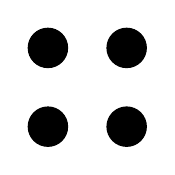
\begin{tikzpicture}
            \filldraw (0,0) circle (0.25cm);
            \filldraw (1,0) circle (0.25cm);
            \filldraw (1,1) circle (0.25cm);
            \filldraw (0,1) circle (0.25cm);
        \end{tikzpicture}
    \end{center}
    Para $n=3$:
    \begin{center}
        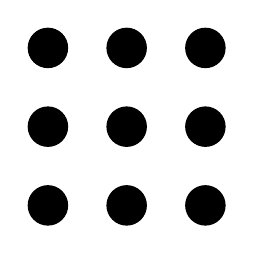
\begin{tikzpicture}
            \filldraw (0,0) circle (0.25cm);
            \filldraw (1,0) circle (0.25cm);
            \filldraw (1,1) circle (0.25cm);
            \filldraw (0,1) circle (0.25cm);
            \filldraw (2,0) circle (0.25cm);
            \filldraw (2,1) circle (0.25cm);
            \filldraw (2,2) circle (0.25cm);
            \filldraw (1,2) circle (0.25cm);
            \filldraw (0,2) circle (0.25cm);
        \end{tikzpicture}
    \end{center}
    Para $n=4$:
    \begin{center}
        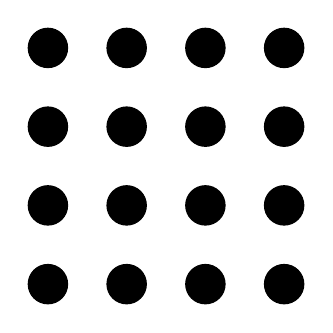
\begin{tikzpicture}
            \filldraw (0,0) circle (0.25cm);
            \filldraw (1,0) circle (0.25cm);
            \filldraw (1,1) circle (0.25cm);
            \filldraw (0,1) circle (0.25cm);
            \filldraw (2,0) circle (0.25cm);
            \filldraw (2,1) circle (0.25cm);
            \filldraw (2,2) circle (0.25cm);
            \filldraw (1,2) circle (0.25cm);
            \filldraw (0,2) circle (0.25cm);
            \filldraw (3,0) circle (0.25cm);
            \filldraw (3,1) circle (0.25cm);
            \filldraw (3,2) circle (0.25cm);
            \filldraw (3,3) circle (0.25cm);
            \filldraw (2,3) circle (0.25cm);
            \filldraw (1,3) circle (0.25cm);
            \filldraw (0,3) circle (0.25cm);
        \end{tikzpicture}
    \end{center}
    \captionsetup*[figure]{font={footnotesize},hypcap=false}%
    \captionof{figure}{Representación del modelo $1+3+5+\cdots +(2n-1)=n^2$ cuando $n = 1$, $2$, $3$, $4$}\label{fig:JEJDJJJJJJDJJ}
    }

    \noindent Por lo que se propone el siguiente modelo:
    $$1+3+5+7+9+11+\cdots +(2n-1)=n^2.$$
    Probemosla por medio de inducción sobre $n$. Llamemos a la suma, $S_n$. Es decir,
    $$S_n=1+3+5+7+9+11+\cdots +(2n-1).$$
    \begin{enumerate}[label=\roman*.]
        \item Para $n=1$ es evidente que se cumple, ya que la suma consiste en un solo término, el $1$. El valor de la expresión $n^2$ también es $1$.
        \item Supóngase que la hipótesis se cumple para $n=k$, es decir, $S_k=k^2$.
        \item A partir de (ii), probemos que se cumple para $n=k+1$, es decir,
        $$S_{k+1}=(k+1)^2.$$
        En efecto, se tiene
        $$S_{k+1}=S_k+(2k+1)$$
        pero $S_k=k^2$, se sigue que
        $$S_{k+1}=k^2+(2k+1)=(k+1)^2$$
    \end{enumerate}
    En conclusión, se cumple que $S_n=n^2$. Incluso, para este caso, podemos ver la \emph{demostración visual} de\infoBulle{Una demostración visual implica que la solución de un problema sea accesible de manera clara a través de un diagrama o dibujo, con un mínimo de desarrollo matemático necesario.}
    $$1+3+5+7+9+11+\cdots +(2n-1)=n^2$$
    como se muestra en la figura \ref{fig:JEJDJJJJJJDJJ}. Aunque no se debe olvidar que esto es una manera visual de ver el comportamiento de una proposición particular. No siempre se puede recurrir a una demostración visual, ya que nos puede llevar a conclusiones falsas.
\end{Problem}

\section{Inducción errónea en las matemáticas}

\begin{example}
    Consideremos el polinomio $f(x)=x^2+x+41$. Si este polinomio se remplaza $x$ por el número $0$, se obtiene el número primo $41$. Si se remplaza $x$ por el número $1$, nuevamente se obtiene un número primo, $43$. Si se sigue este procedimiento para $1$, $2$, $3$, $4$, $5$, $6$; obtenemos que
    \begin{align*}
        f(0) &=41 \\
        f(1) &=43 \\
        f(2) &=47 \\
        f(3) &=53 \\
        f(4) &=61 \\
        f(5) &=71 \\
        f(6) &=83 \\
        f(7) &=97
    \end{align*}
    Basándonos en estos resultados podríamos concluir que para todo entero no negativo $x$, el valor del polinomio es un número primo. Pero esto no es así, pues el polinomio $x^2+x+41$ produce números primos para $f(0)$, $f(1)$, $f(2)$, $f(3)$, $\dots$, $f(38)$, $f(39)$ y al obtener el resultado de $f(40)$, que es $1681$, vemos que es un número compuesto.
\end{example}

\begin{example}
    El binomio $x^n-1$, $n \in \NN$, fue estudiado por numerosos matemáticos y fue resuelto en factores (con coeficientes enteros). Al estudiar dichas factorizaciones para muchos valores particulares de $n$, los matemáticos notaron que, en cada uno de los casos estudiados, los valores absolutos de los coeficientes de los factores nunca excedieron al número $1$. Es decir,
    \begin{align*}
        x-1 &=x-1 \\
        x^2-1 &=(x-1)(x+1) \\
        x^3-1 &=(x-1)\left( x^2+x+1 \right) \\
        x^4-1 &=(x-1)(x+1)\left(x^2+1\right) \\
        &\vdots 
    \end{align*}
    Se construyeron tablas de los coeficientes y, en cada uno de los casos, los coeficientes tenían la propiedad antes mencionada. Sin embargo, fallaron todos los intentos para probar que la proposición era verdadera para todos los valores de $n$. No fue hasta que V. Ivanov resolvió dicho problema en 1941. Si $n<105$, el binomio $x^n-1$ tiene la propiedad anterior. No obstante, uno de los factores de $x^{105}-1$ es el polinomio
    \begin{align*}
        x^{48} & +x^{47}+x^{46}-x^{43}-x^{42}-2x^{41}-x^{40}-x^{39}+x^{36}+x^{35}+x^{34}+x^{33} \\
        &+x^{32}+x^{31}-x^{28}-x^{26}-x^{24}-x^{22}-x^{20}+x^{17}+x^{16}+x^{15}+x^{14} \\
        &+x^{13}+x^{12}-x^9-x^8-2x^7-x^6-x^5+x^2+x+1
    \end{align*}
    que ya no tiene esta propiedad.
\end{example}

\section{El principio de la inducción matemática}

\noindent\textbf{Principio de Inducción Matemática:} Sea $P$ una propiedad cualquiera. Tenemos que $P(1), P(2), P(3), P(4), \dots$ es un conjunto de propiedades para cada número natural tal que:
\begin{enumerate}[label=\roman*.]
    \item $P(1)$ es cierta.
    \item Si $P(n)$ es cierta, entonces $P(n+1)$ es cierta.
\end{enumerate}
Entonces $P(n)$ es cierta para toda $n \in \NN$.

\begin{example}
    Demostrar que
    $$1+2+\cdots +n=\frac{n(n+1)}{2}, \forall n \in \NN.$$\newpage
    \demostracion Claramente $n=1$, satisface la fórmula, ya que
    \begin{align*}
        1 &=\frac{1(1+1)}{2} \\
        1 &=1
    \end{align*}
    lo cual es cierto. Supongamos que la fórmula se cumple para $n=k$, es decir, supongamos que
    $$1+2+\cdots +k=\frac{k(k+1)}{2}.$$
    Demostraremos a partir de lo dicho anteriormente que la fórmula se cumple para $n=k+1$. Es decir, probaremos que
    $$1+2+\cdots +k=\frac{(k+1)(k+2)}{2}.$$
    En efecto, por hipótesis de inducción
    $$1+2+\cdots +k=\frac{k(k+1)}{2}.$$
    Entonces
    \begin{align*}
        1+2+\cdots +k+k+1 &=\frac{k(k+1)}{2}+k+1 \\
        &=\frac{k(k+1)+2(k+1)}{2} \\
        &=\frac{(k+1)(k+2)}{2}
    \end{align*}
    es decir
    $$1+2+\cdots +k+1=\frac{(k+1)(k+2)}{2}.$$
    Por tanto,
    $$1+2+\cdots +n=\frac{n(n+1)}{2}, \forall n \in \NN.$$
\end{example}

\begin{example}
    Demostrar que
    $$1^3+2^3+\cdots +n^3=(1+2 +\cdots +n)^2, \forall n \in \NN.$$
    \demostracion Claramente $n=1$ satisface la fórmula, ya que al sustituir $n$ por $1$ se tiene
    \begin{align*}
        1^3 &=(1)^2 \\
        1 &=1
    \end{align*}
    lo cual es verdadero. Notemos por el ejercicio anterior que
    $$1+2+\cdots +n=\frac{n(n+1)}{2}$$
    entonces tenemos que
    $$1^3+2^3+\cdots +n^3=\left( \frac{n(n+1)}{2} \right)^2.$$
    Así pues, supongamos que la fórmula cumple para $n=k$, es decir
    $$1^3+2^3+\cdots +k^3=\left( \frac{k(k+1)}{2} \right)^2.$$\newpage\noindent
    Demostraremos a partir de lo dicho anteriormente que la fórmula se cumple para $n=k+1$. Es decir, probaremos que
    $$1^3+2^3+\cdots +k^3=\left( \frac{k(k+1)}{2} \right)^2.$$
    En efecto: por hipótesis de inducción
    \begin{align*}
        1^3 +2^3+ \cdots +k^3+(k+1)^3 &=\left( \frac{k(k+1)}{2} \right)^2 +(k+1)^3\\
        &=\frac{k^2(k+1)^2}{4}+(k+1)^3 \\
        &=\frac{k^2(k+1)^2+4(k+1)^3}{4} \\
        &=\frac{(k+1)^2\big(k^2+4(k+1)\big)}{4} \\
        &=\frac{(k+1)^2 (k^2+4k+4)}{4} \\
        &=\frac{(k+1)^2(k+2)^2}{4} \\
        &=\left(\frac{(k+1)(k+2)}{2}\right)^2
    \end{align*}
    Por tanto,
    $$1^3+2^3+\cdots +n^3=(1+2+\cdots +n)^2, \forall n \in \NN.$$
\end{example}

\begin{remark}
    El método de la inducción matemática no es el único procedimiento para demostrar que una propiedad $P$ se cumple para cada número natural.
\end{remark}

\begin{remark}
    Si no se puede demostrar que una propiedad $P$ se cumple para cada número natural, no significa que $P$ sea falsa, sino solamente que no se ha podido hacer la demostración. Una manera de demostrar que $P$ es falsa sería dar un contraejemplo.
\end{remark}

\begin{example}
    Demostrar que
    $$1^2+2^2+\cdots +n^2=\frac{n(n+1)(2n+1)}{6}, \forall n \in \NN.$$
    \demostracion Claramente $n=1$ satisface la fórmula, ya que al sustituir $n$ por $1$ se tiene
    \begin{align*}
        1^2 &=\frac{1(1+1)(2\cdot 1+1)}{6} \\
        1 &=1
    \end{align*}
    lo cual es verdadero. Supongamos que la fórmula se cumple para $n=k$, es decir, supongamos que
    $$1^2+2^2+\cdots +k^2=\frac{k(k+1)(2k+1)}{6}$$
    Demostraremos a partir de lo dicho anteriormente que la fórmula se cumple para $n=k+1$. Es decir, probaremos que
    $$1^2+2^2+\cdots +(k+1)^2=\frac{(k+1)(k+2)(2k+3)}{6}.$$
    En efecto: por hipótesis de inducción
    $$1^2+2^2+\cdots +k^2=\frac{k(k+1)(2k+1)}{6}.$$\newpage\noindent
    Entonces
    \begin{align*}
        1^2 +2^2+\cdots +k^2+(k+1)^2 &=\frac{k(k+1)(2k+1)}{6}+(k+1)^2 \\
        &=\frac{k(k+1)(2k+1)+6(k+1)^2}{6} \\
        &=\frac{(k+1)\big(k(2k+1)+6(k+1)\big)}{6} \\
        &=\frac{(k+1)(2k^2+7k+6)}{6} \\
        &=\frac{(k+1)(k+2)(2k+3)}{6}
    \end{align*}
    Por tanto,
    $$1^2+2^2+\cdots +n^2=\frac{n(n+1)(2n+1)}{6}, \forall n \in \NN.$$
\end{example}

En resumen, cuando se quiere demostrar que una propiedad $P$ se cumple para cada número natural, se emplea un procedimiento llamado \emph{demostración por inducción matemática}. Es decir, si $\NN$ es el conjunto de los números naturales y $A \subset \NN$ tal que:
\begin{enumerate}[label=\roman*.]
    \item $1 \in A$.
    \item $k \in A \Longrightarrow k+1 \in A$. Entonces $A = \NN$.
\end{enumerate}

\section{El principio de inducción modificado}

\noindent\textbf{Principio de Inducción Modificado:} Si $A$ es un subconjunto de los números naturales tal que
\begin{enumerate}[label=\roman*.]
    \item $1 \in A$.
    \item Si $1, 2, \dots , n \in A$, implica que $n+1 \in A$.
\end{enumerate}
    Entonces $A=\NN$.

\begin{observation}
    Sea $P(n)$ una propiedad cualquiera. Si se quiere demostrar que $P(n)$ es cierta para toda $n \in \NN$, es decir,
    $$A:=\left\lbrace n \in \NN \mid P(n) \text{ es cierta} \right\rbrace = \NN$$
    es suficiente mostrar que $A$ satisface las dos hipótesis del Principio de Inducción Modificado.
\end{observation}

\begin{observation}
    Podría suceder que $P(n)$ no sea verdadera para todos los números naturales, pero existe cierto número natural $i$ tal que $P(k)$ es verdadera para toda $i \leq k$. Se puede utilizar también el Principio de Inducción Modificado considerando al conjunto
    $$A:=\left\lbrace n \in \NN \mid P(n+i) \text{ es cierta} \right\rbrace $$
    en cuyo caso se reduce a demostrar que:
    \begin{enumerate}[label=\roman*.]
        \item $P(i)$ es verdadera.
        \item Si $P(k)$ es cierta para $k=i, i+1, \dots, i+n$, entonces $P\big( i+(n+1) \big)$ es cierta.
    \end{enumerate}
\end{observation}

\begin{proposition}
    El Principio de Inducción y el Principio de Inducción Modificado son equivalentes. \\
    \demostracion Se deja como ejercicio al lector.
\end{proposition}

\newpage

\section{El principio de buen orden}

\noindent\textbf{Principio del Buen Orden:} Si $A$ es un subconjunto no vacío de los números naturales, entonces $A$ posee primer elemento (o mínimo), es decir, existe $a \in A$ tal que $a \geq b$, $\forall b \in A$.

\begin{definition}
    Para toda $n \in \NN$, definimos a $S(n)=n+1$ como el sucesor de $n$.
\end{definition}

\begin{definition}
    Para toda $n \in \NN$ tal que $n \geq 1$, definimos el antecesor de $n$ como $n-1$.
\end{definition}

\begin{theorem}
    El Principio de Buen Orden es equivalente al Principio de Inducción. \\
    \demostracion Se deja como ejercicio al lector.
\end{theorem}

\section{Más ejemplos de inducción}

\begin{example}
    Demuestre que
    $$\int_{0}^{\infty} e^{-x}x^{n} dx=n!, \forall n \in \NN.$$
    \demostracion En esta demostración, tomaremos al $0$ como un número natural. Además, recordemos la siguiente propiedad
    $$\lim_{x \to \infty} e^{px}=0, \text{ si } p<0.$$
    Así pues, si $n=0$, entonces
    \begin{align*}
        \int_{0}^{\infty} e^{-x}x^0 dx &= \int_{0}^{\infty} e^{-x} dx \\
        &=\left. -e^{-x} \right|_{0}^{\infty} \\
        &=- \lim_{x \rightarrow \infty} e^{-x} + e^{-0} \\
        &=1 \\
        &=0!
    \end{align*}
    Supongamos que se cumple para $n=k$, es decir,
    $$\int_{0}^{\infty} e^{-x}x^{k} dx=k!.$$
    Demostraremos a partir lo dicho anteriormente, que la propiedad se cumple para $n=k+1$, es decir,
    $$\int_{0}^{\infty} e^{-x}x^{k+1} dx=(k+1)!.$$
    Procederemos por integración por partes. Así pues, tomando a
    $$u=x^{k+1} \quad \text{ y } \quad dv=e^{-x} dx$$
    obtenemos
    $$du=(k+1)x^k dx \quad \text{ y } \quad v=-e^{-x}$$
    Entonces
    \begin{align*}
        \int_{0}^{\infty} e^{-x}x^{k+1} dx &= \left. -x^{k+1}e^{-x} \right|_{0}^{\infty} + (k+1) \int_{0}^{\infty} e^{-x} x^k dx \\
        &=- \lim_{x \rightarrow \infty} x^{k+1}e^{-x}+(0)^{k+1}e^{-0}+(k+1)k! \\
        &=- \lim_{x \rightarrow \infty} \frac{(k+1)!}{e^x} +(k+1)k! \\
        &=(k+1)!
    \end{align*}
    Por tanto,
    $$\int_{0}^{\infty} e^{-x}x^{n} dx=n!, \forall n \in \NN.$$
\end{example}

\begin{example}
    Si $a_1, a_2, \dots, a_n$ son números reales positivos, demuestre que
    \begin{equation}
        \sqrt[n]{a_1\cdot a_2 \cdots a_n} \leq \frac{a_1+a_2+\cdots +a_n}{n}. \label{A1}
    \end{equation}
    \demostracion \sideFigure[\label{fig:JNVKJYYS}]{
    \begin{center}
        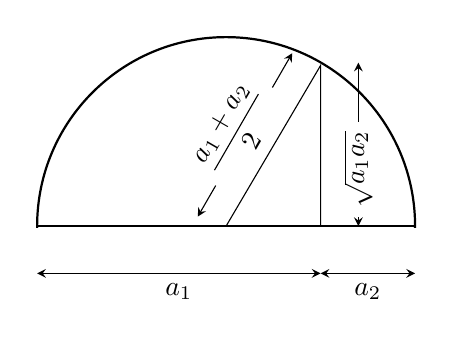
\begin{tikzpicture}[baseline=(current bounding box.north),scale=1.2]
            \begin{scope}
                \clip (-2.1,-0.01) rectangle (2.1,2.1);
                \draw[thick] (0,0) circle (2);
                \draw[thick] (-2,0) -- (2,0);
                \draw (1,0) -- (1,1.7) -- (0,0);
                \draw[stealth-stealth] (1.4,0) -- (1.4,1.73);
                \node[fill=white,rotate=90] at (1.4,0.6) {$\sqrt{a_1a_2}$};
            \end{scope}
            \draw[stealth-stealth] (-2,-0.5) -- (1,-0.5);
            \node at (-0.5,-0.5) [below] {$a_1$};
            \draw[stealth-stealth] (1,-0.5) -- (2,-0.5);
            \node at (1.5,-0.5) [below] {$a_2$};
            \draw[stealth-stealth] (-0.3,0.1) -- (0.7,1.83);
            \node[fill=white,rotate=60] at (0.1,1) {$\displaystyle \frac{a_1+a_2}{2}$};
        \end{tikzpicture}
    \end{center}
    }
    \begin{enumerate}[label=\roman*.]
        \item Para $n = 2$, la desigualdad \eqref{A1} da
        \begin{equation}
            \sqrt{a_1a_2} \leq \frac{a_1+a_2}{2}. \label{A2}
        \end{equation}
        Es fácil obtener esta desigualdad a partir de esta otra
        $$\left( \sqrt{a_1} - \sqrt{a_2} \right)^2 \geq 0,$$
        válida para cualesquiera $a_1$, $a_2$ números reales positivos. Notemos que la desigualdad \eqref{A2} admite una interpretación geométrica sencilla. Tomemos sucesivamente en una recta $AB$ los segmentos $a_1$ y $a_2$. Construyamos la circunferencia cuyo diámetro es la suma de estos segmentos. Entonces, $\displaystyle \frac{a_1+a_2}{2}$ es el radio de esta circunferencia y $\sqrt{a_1a_2}$ es la mitad de la cuerda perpendicular al diámetro en el punto común de los segmentos $a_1$ y $a_2$ (vea la figura \ref{fig:JNVKJYYS}); de aquí se deduce la desigualdad \eqref{A2}.
        \item Supongamos que la desigualdad \eqref{A1} se cumple para $n = k$. Demostremos que, entonces, también se cumple para $n = 2k$. En efecto,
        \begin{align*}
            \sqrt[2k]{a_1\cdot a_2 \cdots a_{2k}} & = \sqrt{\sqrt[k]{a_1 \cdot a_2 \cdots a_k}\sqrt[k]{a_{k+1} \cdots a_{2k}}} \\
            & \leq \frac{\sqrt[k]{a_1 \cdot a_2 \cdots a_k} + \sqrt[k]{a_{k+1} \cdots a_{2k}}}{2} \\
            & \leq \displaystyle\frac{\displaystyle\frac{a_1+a_2+\cdots +a_k}{k} +\displaystyle\frac{a_{k+1}+\cdots+a_{2k}}{k}}{2} \\
            & = \frac{a_1+a_2+\cdots+a_k+\cdots+a_{2k}}{2k}
        \end{align*}
        Puesto que hemos demostrado ya la desigualdad \eqref{A1} para $n = 2$, podemos afirmar ahora que de cumple para $n = 4$, $8$, $16$, etc., o sea, para $n = 2^s$, donde $s$ es un número natural.
        \item Para demostrar que la desigualdad \eqref{A1} se cumple para cualquiera que sea el número natural $n$, probemos que si se cumple para $n = k$, también se cumple para $n = k-1$.
        
        Sean pues, $a_1$, $a_2$, $\dots$, $a_{k-1}$ números reales positivos. Sea $\lambda$ un número real positivo, entonces
        $$\sqrt[k]{a_1 \cdot a_2 \cdots a_{k-1}\lambda} \leq \frac{a_1+a_2+\cdots+a_{k-1}+\lambda}{k}.$$
        Determinemos $\lambda$ de modo que
        $$\frac{a_1+a_2+\cdots+a_{k-1}+\lambda}{k} = \frac{a_1+a_2+\cdots+a_{k-1}}{k-1},$$
        o sea, pongamos
        $$\lambda = \frac{a_1+a_2+\cdots+a_{k-1}}{k-1}.$$\newpage
        Tenemos
        $$\sqrt[k]{\frac{a_1 \cdot a_2 \cdots a_{k-1} (a_1+a_2+\cdots+a_{k-1})}{k-1}} \leq \frac{a_1+a_2+\cdots+a_{k-1}}{k-1},$$
        es decir,
        $$\sqrt[k-1]{a_1 \cdot a_2 \cdots a_{k-1}} \leq \frac{a_1+a_2+\cdots+a_{k-1}}{k-1}.$$
        Sea ahora $m$ un número natural cualquiera. Si $m = 2^s$, la desigualdad se cumple en virtud de (ii). Si $m \neq 2^s$, determinemos el número $s$ de modo que $m$ sea menor que $2^s$; entonces, basándonos en (ii) y (iii), podemos afirmar que la desigualdad se cumple para $n = m$.
    \end{enumerate}
    Por tanto, se cumple que\infoBulle{Obsérvese que si $a_1 = a_2 = \cdots = a_n$, entonces $$\sqrt[n]{a_1\cdot a_2 \cdots a_n} = \frac{a_1+a_2+\cdots +a_n}{n}.$$En caso contrario, $$\sqrt[n]{a_1\cdot a_2 \cdots a_n} < \frac{a_1+a_2+\cdots +a_n}{n}.$$ para cualesquiera $a_1$, $a_2$, $\dots$, $a_n$ números reales positivos}
    $$\sqrt[n]{a_1\cdot a_2 \cdots a_n} \leq \frac{a_1+a_2+\cdots +a_n}{n}, \forall a_1, a_2, \dots, a_n \in \RR[+], \forall n \in \NN.$$
\end{example}

\begin{example}
    Hallar una expresión para la suma
    $$1 \cdot 1! + 2 \cdot 2! + 3 \cdot 3! + \cdots + n \cdot n!.$$
    \demostracion Llamemos a la suma anterior, $S_n$. Es decir
    $$S_n=1 \cdot 1! + 2 \cdot 2! + 3 \cdot 3! + \cdots + n \cdot n!.$$
    Veamos las siguientes sumas parciales
    \begin{align*}
        1 \cdot 1! &=1 \\
        1 \cdot 1!+2 \cdot 2! &=5 \\
        1 \cdot 1!+2 \cdot 2! + 3 \cdot 3! &=23 \\
        1 \cdot 1!+2 \cdot 2! + 3 \cdot 3! +4 \cdot 4! &=119
    \end{align*}
    Examinando las anteriores sumas, se observa que
    \begin{align*}
        S_1 &=2!-1 \\
        S_2 &=3!-1 \\
        S_3 &=4!-1 \\
        S_4 &=5!-1
    \end{align*}
    Esto conduce a la hipótesis
    $$S_n=(n+1)!-1.$$
    Verifiquemos dicha hipótesis.
    \begin{enumerate}[label=\roman*.]
        \item La hipótesis se cumple para $n=1$, pues
        $$S_1=1 \cdot 1!=2!-1.$$
        \item Supongamos que la hipótesis se cumple para $n=k$, es decir,
        $$S_k=(k+1)!-1.$$
        \item A partir de (ii), probemos que se cumple para $n=k+1$, es decir,
        $$S_{k+1}=(k+2)!-1.$$
        En efecto,
        \begin{align*}
            S_{k+1} &= S_k + (k+1) \cdot (k+1)! \\
            &=[(k+1)!-1]+(k+1) \cdot (k+1)! \\
            &=(k+1)![1+(k+1)]-1 \\
            &=(k+1)!(k+2)-1 \\
            &=(k+2)!-1
        \end{align*}
    \end{enumerate}
    Por tanto,
    $$1 \cdot 1! + 2 \cdot 2! + 3 \cdot 3! + \cdots + n \cdot n! = (n+1)!-1.$$
\end{example}

\newpage

\section{Ejercicios}

\begin{enumerate}
    \item Demostrar que
    $$1^2+3^2+\cdots +(2n-1)^2=\frac{4n^3-n}{3}, \forall n \in \NN.$$
    \item Demostrar que
    $$\frac{1}{1\cdot 2}+\frac{1}{2\cdot 3}+\frac{1}{3\cdot 4}+\cdots +\frac{1}{n(n+1)}=\frac{n}{n+1}, \forall n \in \NN.$$
    \item Demostrar que
    $$\frac{1}{1\cdot 3}+\frac{1}{3\cdot 5}+\frac{1}{5\cdot 7}+\cdots +\frac{1}{(2n-1)(2n+1)}=\frac{n}{2n+1}, \forall n \in \NN.$$
    \item Demostrar que
    $$2^n>n, \forall n \in \NN.$$
    \item Demostrar que
    $$1^2-2^2+3^2-4^2+\cdots +(-1)^{n-1}n^2=(-1)^{n-1} \frac{n(n+1)}{2}, \forall n \in \NN.$$
    \item Demostrar que para toda $n \in \NN$
    $$1 \cdot 2 \cdot 3 + 2\cdot 3 \cdot 4 + \cdots + n(n+1)(n+2) = \frac{n(n+1)(n+2)(n+3)}{4}.$$
    \item Demostrar que para toda $n \in \NN$, $n>1$
    $$\frac{1}{n+1}+\frac{1}{n+2}+\cdots +\frac{1}{2n}>\frac{13}{24}.$$
    \item Demostrar que para toda $n \in \NN$, $n>1$
    $$\frac{1}{\sqrt{1}}+\frac{1}{\sqrt{2}}+\cdots +\frac{1}{\sqrt{n}}>\sqrt{n}.$$
    \item Demostrar que para toda $n \in \NN$
    $$1+2n \leq 3^n.$$
    \item Demuestre que $(n-1)^2 \mid n^{n-1}-1$ para toda $n \in \NN$, $n>1$.
    \item Demuestre que $n^2+n$ es un número par para toda $n \in \NN$.
    \item Demuestre que $8^n-3^n$ es múltiplo de $5$ para toda $n \in \NN$.
    \item Demuestre que $n^3-n$ es múltiplo de $6$ para toda $n \in \NN$.
    \item Demuestre que $2^{2n-1}+3^{2n-1}$ es múltiplo de $5$ para toda $n \in \NN$.
    \item Demuestre que $11^{n+1}+12^{2n-1}$ es múltiplo de $19$ para toda $n \in \NN$.
    \item Si $a \neq 1$, entonces
    $$1+a+a^2+\cdots +a^n=\frac{a^{n+1}-1}{a-1}, \forall n \in \NN.$$
    \item Demuestre que
    $$3+3^2+3^3+\cdots +3^n=\frac{3(3^n-1)}{2}, \forall \in \NN.$$\newpage
    \item Demostrar por inducción
    $$1+nx \leq (1+x)^n, \forall n \in \NN, x \geq -1.$$
    Esta desigualdad es conocida como desigualdad de Bernoulli.
    \item Demuestre que el número $S_n$ de permutaciones de $n$ elementos está dado por
    $$S_n=n!.$$
    \item Demuestre que si $a \neq b$, entonces el siguiente determinante de $n \times n$ se cumple:
    $$
    \begin{vmatrix}
        a+b & ab & 0 & \cdots & 0 & 0 \\
        1 & a+b & ab & \cdots & 0 & 0 \\
        0 & 1 & a+b & \ddots & 0 & 0 \\
        \vdots & & & \ddots & \\
        0 & 0 & 0 & \ddots & a+b & ab \\
        0 & 0 & 0 & \cdots & 1 & a+b
    \end{vmatrix} = \frac{a^{n+1}-b^{n+1}}{a-b}.
    $$
    \item Probar la identidad
    $$\cos (\varphi) \cos (2\varphi) \cos (4\varphi) \cdots \cos \left( 2^n \varphi \right)=\frac{\sen \left( 2^{n+1} \varphi \right)}{2^{n+1} \sen (\varphi)}.$$
    \item Probar que
    $$\frac{1}{2}+\cos x +\cos 2x +\cdots +\cos nx=\frac{ \sen \frac{2n+1}{2}x}{2\sen \frac{x}{2}}.$$
    \item Demuestre que
    $$\frac{d^n}{dx^n}\left( \frac{\sen x}{x} \right) = \frac{1}{x^{n+1}} \int_{0}^{x} y^n \cos \left( y+\frac{n\pi}{2} \right) dy, \forall n \in \NN.$$
    \item Demuestre que
    $$\binom{n}{0}+\binom{n}{1}+\cdots +\binom{n}{n}=2^n, \forall n \in \NN.$$
    \item Sea $n$, $k \in \NN$ con $0 \leq k \leq n$, demuestre que
    $$\binom{k}{k}+\binom{k+1}{k}+\binom{k+2}{k}+\cdots +\binom{n}{k}=\binom{n+1}{k+1}.$$
\end{enumerate}